\documentclass[conference]{IEEEtran}
\IEEEoverridecommandlockouts
% The preceding line is only needed to identify funding in the first footnote. If that is unneeded, please comment it out.
\usepackage{cite}
\usepackage{amsmath,amssymb,amsfonts}
\usepackage{algorithmicx}
\usepackage{graphicx}
\usepackage{textcomp}
\usepackage{paralist}
\usepackage{tikz-cd}
\usepackage{tikz}
\usepackage{wrapfig}
\usepackage{amssymb}
\usepackage{mathrsfs}
\usepackage{dsfont}
\usepackage{proof}
%\usepackage[cmex10]{amsmath}
\usepackage{stmaryrd}
\usepackage{subfigure}
\usepackage{algpseudocode}
\usepackage{enumitem}
%\usepackage{algorithm}

\newtheorem{Definition}{Definition}
\newtheorem{Theorem}{Theorem}
\newtheorem{Lemma}{Lemma}
\newtheorem{Example}{Example}
\newtheorem{Corollary}{Corollary}
\def\BibTeX{{\rm B\kern-.05em{\sc i\kern-.025em b}\kern-.08em
    T\kern-.1667em\lower.7ex\hbox{E}\kern-.125emX}}
\begin{document}

\title{\hspace*{-6mm}\begin{minipage}{1.1\linewidth}Verified Model Refactorings for Hybrid Control Systems\end{minipage}}
%\subtitle{Extended Abstract for PhD Thesis}
\author{\IEEEauthorblockN{Sebastian Schlesinger}
\IEEEauthorblockA{Software and Embedded Systems Engineering\\
Technische Universit\"at Berlin, Germany\\
%Ernst-Reuter-Platz 7, 10587 Berlin\\
Email: sebastian.schlesinger@tu-berlin.de}}
\maketitle

\subsection*{Problem Statement}

%Embedded systems nowadays are ubiquitous and of high complexity. 
The ever growing complexity in modern embedded systems requires to incorporate increasingly many functions into a single system. %Such increasing functionality leads to growing design complexity. 
Model Driven Engineering (MDE) is a well-established technique for the development of such complex embedded systems. 
Refactoring is a common technique to reduce the complexity and establish compliance with industrial MDE guidelines via model transformations. However, model refactorings are often performed manually or partially automatically via tools without guarantee of correctness. Such refactorings therefore bear the risk of introducing unwanted or even erroneous behaviour. This is critical, especially in safety-critical applications, where an error may cause enormous costs or even endanger human lifes. To overcome this problem, I present an approach to guarantee behavioural equivalence of graph-based hybrid control systems.
%In this dissertation we tackle the problem of guaranteeing the correctness of refactorings on graph-based hybrid control systems. 

%Behavioural equivalence is the key property that needs to be guaranteed by a correct refactoring. 


\subsection*{Challenges}
The key challenges we address with our approach are:
\begin{itemize}[itemsep=0pt]
\item \emph{Hybrid Systems:} We consider models comprising time-discrete, time-continuous, and control flow elements together. The time-continuous part introduces an approximation error caused by the execution on machines with finite execution time and storage space. The challenges are firstly to properly consider this approximate nature  of time-continuous model parts, secondly to consider the interplay of data flow and control flow in the models, and thirdly to consider discrete jumps in continuous behaviour.%possible time-delays at switches.
\item \emph{Formal Foundation:} To provide guarantees for all possible input scenarios, a precise mathematical description is required.  %Since we aim for a formal verification approach, we require a formal foundation. 
However, Simulink has only an informal, descriptive semantics. We require a precise and formal semantics and equivalence notion.
\item \emph{Automation:} A manual approach requires an unacceptable amount of effort for verification and its application is likely to be erroneous. A largely automated solution is therefore desired. However, this is challenging because the state space for hybrid control systems gets extremely large for arbitrary input signals.
\end{itemize}

% \subsection*{Criteria}
% Our criteria for the targeted solution are:
% A formal foundation comprising a) a formal, precise, and unambiguous semantics for a hybrid control systems language, b) a formal equivalence notion, and c) a formal and automatable proof scheme.
% Our approach must be able to handle the approximate nature of the semantics.
% We want to support verification of refactorings for time-discrete, time-continuous, time-hybrid, and hybrid data flow-oriented control systems.
% Our solution should provide semi-automated support.
% We want our solution to be applicable to industrially relevant models.
\subsection*{Main Contributions}
Our proposed solution is twofold. Firstly, we provide a framework for the formal verification of refactorings of data-flow oriented hybrid control models. We select MATLAB/ Simulink as most prominent representative of languages for such types of models. 
Secondly, we provide an automation of our framework for a clearly defined subset of Simulink models. 
\begin{figure}
	
 	\centering
	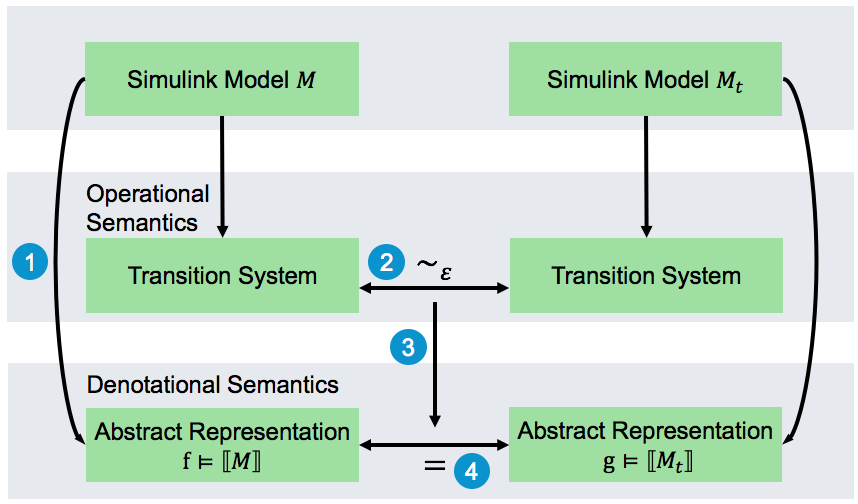
\includegraphics[scale=0.3]{Figures/Approach.PNG}

 	\caption{Overview over the Equivalence Proof Framework}
 	\label{fig:Approach}
 \end{figure}
Figure \ref{fig:Approach} provides an overview over our main contributions. We go through the main contributions as depicted in the figure.

\begin{enumerate}[itemsep=0pt]
\item To obtain a \emph{formal foundation}, we have adopted the approach \cite{Bouissou.2012}, which describes an operational semantics for Simulink. In addition, we provide a semantics on denotational level, which we call the Abstract Representation (AR), and have shown that it is sound with respect to the operational semantics.
%We lift the operational semantics to a denotational level. To this end, 
We automatically extract the AR from a given Simulink model. The AR describes time-discrete parts in terms of difference equations, and time-continuous parts in terms of ordinary differential equations (ODEs). 
%We perform this step because verification of behavioral equivalence requires to compare complete traces or trajectories that the execution yield rather than comparing single steps - as this would be the case by using the operational semantics directly. 
We prove the soundness of our AR with the operational semantics in the following sense: If we consider sequences of executions of the operational semantics with decreasing sample step size, these sequences converge uniformly to the interpretations or solutions determined by the AR.
Our AR is formally well-defined and concise, and it enables us to formally relate traces or trajectories with respect to behavioural equivalence.

\item The simulation semantics of Simulink includes numerical approximations. This means that  
two \emph{hybrid models} that are mathematically equivalent do not necessarily yield exactly the same trajectories if executed on a machine with finite sample step sizes. Therefore, traditional equivalence notions such as bisimulation are not applicable. We therefore adapt the concept of approximate bisimulation to Simulink. Approximate bisimulation allows us to relate two models that are close to each other up to a maximal distance $\varepsilon$, the precision of the approximate bisimulation.

\item We provide a proof scheme, i.e., an approach for automated generation of proof obligations to show approximate bisimulation for time-discrete, time-continuous, and hybrid models. The proof obligations are provided on a denotational, mathematical level. We also provide means to automatically calculate the \emph{precision $\varepsilon$} of the approximate bisimulation.
%The fifth contribution is an extension of the operational semantics enabling support for blocks and refactorings with industrial relevance.


\item We provide an approach for \emph{semi-automated verification} of behavioral equivalence of data flow-oriented hybrid control systems expressed by linear difference and differential equations. Our automation approach is %an application of our framework. 
%It comprises firstly
based on a calculation of all possible data flow paths in a given model. We call them Data Flow Models. Each Data Flow Model does not contain control flow elements, i.e., we eliminate control flow elements such as Switch blocks from the original model and calculate a set of models without control flow. 
Then, we partition the Data Flow Models to enable modular verification. The partitioning distinguishes between cycles or feedback loops and non-cyclic or directed cyclic graph (DAG) elements. %We require the partitions within the partitioning to be either purely time-discrete or time-continuous and allow only linear difference equations or ODEs there. 
We extract the ARs of the partitions for all Data Flow Models and verify their equivalence symbolically. In this step, we make use of Laplace- and z-transform to transform the system into simple algebraic expressions rather than complex ODEs. This enables largely automated symbolic equivalence verification with the help of a Computer Algebra System (CAS). The only manual interaction that is required is a mapping of partitions from the original to the refactored model. %Within the Data Flow Models, we follow an assume-guarantee approach to verify the equivalence of all partitions. 

We provide an approach to automatically calculate the local precision $\varepsilon_l$, i.e., the disturbance resulting from the approximation at the partition where the refactoring took place. 
We propagate the local precision $\varepsilon_l$ to a global precision $\varepsilon_g$. The global precision is the overall precision of the approximate bisimulation of source and target model. %We propagate the local precision by providing estimates for subsequent partitions in the Data Flow Models under consideration of local disturbances being carried over.

Finally, we verify supplemental proof obligations such as conditions that exclude time-delayed behaviour at control flow elements, or conditions to guarantee injectivity of Laplace or z-transform. 
\end{enumerate}
We have published our framework for purely time-discrete and purely time-continuous models in \cite{Schlesinger.2015,Schlesinger.2016} and for hybrid control systems in \cite{Schlesinger.CyPhy}. 
We have demonstrated the practical applicability of our approach with various case studies, comprising industrial Simulink examples from The MathWorks, Inc. as well as case studies from our industrial partners from the automotive industry.

\subsection*{Related Work}
%We divide related work in five categories and provide an extract for each of them. 
There are various articles concerning formal Simulink verification, e.g. \cite{Reicherdt.2014,.2013b,Tripakis.2005}. In each of them, the authors map only a subset of Simulink to formal languages. Some work has been published to formalise semantics of causal block diagrams in general or Simulink in particular, e.g. \cite{Bouissou.2012,gomes2016causal,dragomir2016compositional}. However, they do not consider formal verification of behavioural equivalence. We have chosen and extended \cite{Bouissou.2012} as our formal foundation. There exists a large variety of works about hybrid systems verification, e.g. \cite{fulton2015keymaera,alur2011formal}, and on behavioural equivalence of hybrid systems, e.g. \cite{Girard.2011}. However, they do not consider the specifics of data flow-oriented hybrid control modelling languages such as Simulink. Finally, there exist some works on refactorings of Simulink models, e.g. \cite{.2013}. However, they do not aim at verification of behavioural equivalence. 


\subsection*{Conclusion}
In my thesis, I have provided a framework for formal verification of behavioural equivalence of data-flow oriented hybrid control systems. I have automated the approach for a clearly defined subsystem of the most prominent representative of such models, namely Simulink. %Our approach enables to verify correctness of model refactorings, which is a major challenge in embedded systems design. 
With this approach, introduction of erroneous behaviour during refactorings is avoided. It therefore is a substantial contribution to increase safety in embedded systems design.
\bibliographystyle{alpha}
\bibliography{lit}


%%%%%%%%%%%%%%%%%%%%%%%%%%%%%%%%%%%%%%%%%%%%%%%%%%%%%%%%%%%%%%%%%%%%%%%%%%%%%%%

\end{document}
